\documentclass[11pt]{article}
\setlength{\topmargin}{-2.5cm}
\setlength{\headheight}{0in}
\setlength{\textheight}{24.5cm}
\setlength{\textwidth}{18.5cm}
\setlength{\oddsidemargin}{-0.5cm}
\setlength{\evensidemargin}{-0.5cm}

\setlength{\parindent}{0pt}
%\renewcommand{\thesection}{\arabic{section}.\hspace{-0.2em}}

\usepackage{graphicx}
\usepackage{amsmath,amsfonts,amssymb}
\usepackage{array}
\usepackage[colorlinks,urlcolor=blue]{hyperref}

\begin{document}

\title{\bf AMA3020 Short Investigations}
\author{Connor Ballance and Mauro Paternostro} 
\date{\today}
\maketitle

Guidance will be provided by Dr Ballance and Prof Paternostro.
Topics chosen for the pair investigations will generally not be available for the solo investigations.
In a large class, some projects will probably be chosen by more than one
pair or more than one student. However, we would like the class to do as
many {\it different} projects as possible. Although your preferences will be
taken into account, there is no guarantee that you will always be assigned
a project of your first choice.

\setlength{\parskip}{-3pt}

\tableofcontents

\setlength{\parskip}{0pt}

\newpage

\section{The simple pendulum\\ \small{(Pathway: AMA; Pre-requisite: Classical Mechanics)}}
\section{The simple pendulum\\ \small{(%Pathway: AMA; 
Pre-requisite: Classical Mechanics)}}
%\item
%\underline{\large\bf The simple pendulum} \\[0.1cm]
The bob of a simple pendulum of length $l$ moves in accordance with the
differential equation 
\begin{displaymath}
\ddot{\theta} + \frac{g}{l} \sin \theta = 0,
\end{displaymath}
where $\theta$ is the angle the pendulum makes with the vertical and $g$ is
the acceleration due to gravity. The most elementary approach in classical mechanics books considers only small
oscillations for which  $|\theta | \ll 1$ (in radians, of course!). In this
case $\sin \theta \simeq \theta $ and the equation describes simple harmonic
motion,
\begin{displaymath}
\theta (t)= a \cos (\omega t + \alpha ),
\end{displaymath}
with the amplitude $a$, initial phase $\alpha $, angular frequency
$\omega = \sqrt{g/l}$ and period $T=2\pi /\omega $.\\[6pt]
What happens if $\theta$ is not small?


\section{No one should miss a penalty!\\ \small{(Pathway: Any; Pre-requisite: None)}}
\section{No one should miss a penalty!\\ \small{(%Pathway: Any; 
Pre-requisite: None)}}
%\item
%\underline{\large\bf No one should miss a penalty!} \\[0.1cm]
By tradition, the penalty spot in football is 12 yards (36 feet) from the
centre of the goal which measures 24 feet wide by 8 feet high.\\[6pt]
Is this the best position to maximise the chance that a goal is scored?


\section{At the rising of the Sun\\ \small{(Pathway: Any; Pre-requisite: None)}}
\section{At the rising of the Sun\\ \small{(%Pathway: Any; 
Pre-requisite: None)}}
%\item
%\underline{\large\bf At the rising of the Sun} \\[0.1cm]
The number of hours of daylight varies with the time of the year and is
different at different latitudes, because the axis of rotation of the Earth
is not perpendicular to the plane of the Earth's orbit around the Sun. (The
axial tilt is $\alpha =23.5^\circ $.) Devise a method that allows one to
determine the length of daylight at any point on the Earth's surface at
any time of the year.\\[6pt]
Can you also find the times of sunrises and sunsets?


\section{Loose chippings\\ \small{(Pathway: Any; Pre-requisite: None)}}
\section{Loose chippings\\ \small{(%Pathway: Any; 
Pre-requisite: None)}}
%\item
%\underline{\large\bf Loose Chippings} \\[0.1cm]
Many local authorities recommend that car drivers limit the speed of the car
to 20~mph when travelling over roads which have been newly surfaced with
bituminous binder and stone chippings. The advisory limit is intended to
avoid the situation where loose stones lifted by the rear wheels of a vehicle
in front fly into the path of your vehicle and can cause damage to paintwork
or even break the windscreen.\\[6pt]
Investigate whether this is a reasonable speed limit, given that the
vehicles are separated by a distance recommended by the Highway Code (i.e.,
a two-second gap).
\\[6pt]
You may assume that relative to the vehicle the stones are projected with the
speed of the vehicle,
%that the flying stones remain in the vertical plane containing the motion of
%the vehicle, that vehicles travel at constant speed, 
that air resistance is negligble and that drivers are only worried about
stones hitting the front of the bonnet (typically 0.75 metres above the
ground). Any other assumptions which you make should be stated clearly.


\section{Stiff differential equations\\ \small{(Pathway: Any; Pre-requisite: None, but familiarity with coding would help)}}
\section{Stiff differential equations\\ \small{(%Pathway: Any; 
Pre-requisite: None, but familiarity with coding would help)}}
%\item
%\underline{\large\bf Stiff differential equations} \\[0.1cm]
Many differential equations that are of importance in mathematics and its
applications can only be solved numerically. In this case one must ensure that
the solution obtained is {\em accurate}. In particular, errors can occur when
solutions contain terms that decrease rapidly. This problem can be illustrated
by the following equation
\begin{displaymath}
\frac{dx}{dt} = -30x,
\end{displaymath}
that needs to be solved with the initial conditions $x(0)=1$.
\begin{itemize}\setlength{\itemsep}{0pt}
\item Calculate the estimated value of $x(h)$ using a single step of the
Runge-Kutta method of order 4 for various step sizes $h$ and compare with the
exact result.
\item Use the scipy differential equation solver {\tt vode}
with integrator option {\tt `bdf'} (stiff problems) and {\tt `adams'} (non-stiff problems) to find numerical
solutions and compare them with the exact result.
\item Repeat the last two steps for
\begin{displaymath}
\dot x=-20x+20\sin \omega t + \omega \cos \omega t
\end{displaymath}
What happens for $\omega =0.02$? What happens for other values of $\omega $?
\end{itemize}
See also {\it Numerical Analysis} by R.~L.~Burden and J.~D.~Faires.



\section{Fibonacci and related numbers\\ \small{(Pathway: AMA; Pre-requisite: None)}}
\section{Fibonacci and related numbers\\ \small{(%Pathway: AMA; 
Pre-requisite: None)}}
%\item
%\underline{\large\bf Fibonacci and related numbers} \\[0.1cm]
{\em Fibonacci numbers} $\{F_n\}$ satisfy the recurrence relation
\begin{displaymath}
F_{n+2} =  F_{n+1}+F_n \qquad (n \geq 1),
\end{displaymath}
with $F_1=F_2=1$.  They are given explicitly by Binet's formula
\begin{equation}\label{eq:Fib}
F_{n} = \frac{\alpha^n - \beta^n}{\sqrt 5},
\end{equation}
where $\alpha, \beta$ are the roots of $x^2 -x - 1$ = 0. \\[6pt]
{\em Lucas numbers} $\{L_n\}$ satisfy the same recurrence relation
\begin{displaymath}
L_{n+2} = L_{n+1}+L_n \qquad (n \geq 1),
\end{displaymath}
but have $L_1=1$, $L_2=3$.
\begin{itemize}\setlength{\itemsep}{0pt}
\item Find an expression for $L_n$ similar to that for $F_n$, given by
Eq.~(\ref{eq:Fib}).
\item Show that $F_{n+2}+F_n=L_{n+1}$.
\item Consider other relations involving these number sequences.
\item Consider other related sequences.
\end{itemize}

A related problem (suggested by Dr Alex Schuchinsky) is to consider a sequence
of ``words'' constructed from two symbols, say $a$ and $b$, in which the next
member of the sequence is constructed by concatenating the two previous
``words''. Starting from the two smallest ``words'', i.e., $a$ and $b$, one
obtains
\[
a,~b,~ab,~bab,~abbab,~bababbab,~\text{etc.}
\]
As one can see, the length of the $n$th word in the sequence is $F_n$.
One can also notice that starting from the fifth member, the ``words'' contain
at least one ``double-b'', i.e., $bb$. Is it possible to determine,
how many $bb$'s are in the $n$th ``word''?

% Solution: The recurrency relation for the number of ``double-bes'' is
% $B_{2n+1}=B_{2n}+B_{2n-1}+1$ and $B_{2n}=B_{2n-1}+B_{2n-2}$. Using these
% one can show that $B_{2n+1}=3B_{2n-1}-B_{2n-3}$ that links three
% conseciuitive odd member of the sequence. Solving this, and using
% the ``initial conditions'' $B_3=0$, $B_5=1$, one obtains:
% $B_{2n+1}=(p^{n-1}-q^{n-1})\sqrt{5}$, where $p=(3+\sqrt{5})/2$
% and $q=(3-\sqrt{5})/2$ are the two roots of the quadratic equation
% $x^2-3x+1=0$. Even members of the series can be found from the recurrency
% relation formula $B_{2n}=B_{2n+1}-B_{2n-1}-1$.




\section{Dipsticks\\ \small{(Pathway: Any; Pre-requisite: None)}}
\section{Dipsticks\\ \small{(%Pathway: Any; 
Pre-requisite: None)}}
%\item
%\underline{\large\bf Dipsticks} \\[0.1cm]
A domestic tank which can hold 1000 litres of heating oil is in the shape of
a right circular cylinder, with its axis horizontal. Calibrate a dipstick to
show marks at intervals of 50 litres.
 

\section{Circles on a lattice\\ \small{(Pathway: Any; Pre-requisite: None)}}
\section{Circles on a lattice\\ \small{(%Pathway: Any; 
Pre-requisite: None)}}
% Circles on a lattice
Consider all points with integer coordinates on the $xy$ plane, such as
$(0,0)$, $(1,0)$, $(-2,5)$, etc. These points form a
square lattice. A circle of radius $R$ centered at the origin may pass
through a number of lattice points for some values of $R$, while for others
it will pass through none. For example, for $R = \sqrt{2}$ the circle contains
four lattice points: $(\pm 1,\pm 1)$, but for $R = 3/2$ no lattice points lie
on the circle.\\[6pt]
It is easy to see that for a circle to contain any lattice points, its
radius must be the square root of a natural number, i.e., $R=\sqrt{n}$,
where $n\in \mathbb{N}$. However, this condition is not sufficient, e.g.,
the circle with $R =\sqrt{3}$ contains no lattice points, while that with
$R=\sqrt{5}$ contains a few (how many?).\\[6pt]
Investigate this problem. The aim is to find out as much as possible about
the number of lattice points that a circle may pass through, as a function of
$n$. In particular, can we say anything about the {\em average} number of
lattice points per circle?



\section{Cycling into the wind\\ \small{(Pathway: AMA; Pre-requisite: Classical Mechanics)}}
\section{Cycling into the wind\\ \small{(%Pathway: AMA; 
Pre-requisite: Classical Mechanics)}}
%\item
%\underline{\large \bf Cycling into the wind}\\[0.1cm]
It often seems that you are more likely to cycle into the wind than to have the
wind in your back. While cynics may say that this is a purely psychological
effect of the effort you make to overcome the wind, good modelling
suggest that the effect is due to air resistance.
\begin{itemize}\setlength{\itemsep}{0pt}
\item Assume that the air is a collection of particles which move in the same
direction and the same (wind) speed. How does the air resistance depend on
the wind speed, the cyclist's speed and the angle between the direction
of the wind and that of the cyclist?

\item If a cyclist can reach a speed of 20 mph in the absence of any wind, and
25 mph with wind fully in the back, what maximum speed will the cyclist reach
in full headwind? What speed can be reached for other wind directions?

\item What effect does resistance due to the road surface have?

\end{itemize}


\section{Bungee jumping\\ \small{(Pathway: Any; Pre-requisite: Classical Mechanics)}}
\section{Bungee jumping\\ \small{(%Pathway: Any; 
Pre-requisite: Classical Mechanics)}}
%\item
%\underline{\large \bf Bungee jumping}\\[0.1cm]
In bungee jumping, a person jumps from a tall structure, e.g., a bridge,
while attached to a long, heavy elastic band. The elastic band ensures that the
person does not hit the surface below. The aim of this project is to find
the acceleration the person experiences while falling.\\[6pt]
To simplify the problem, you can replace the elastic band with a (non-elastic)
rope. Assume also that the rope initially hangs down from the structure
and the person.
\begin{itemize}\setlength{\itemsep}{0pt}
\item How does the speed of the person depend on the distance travelled?
Determine the acceleration of the person by taking the derivative of the
velocity with respect to time. How does it compare to $g$? [Hint: use energy
conservation.] 
\item What happens for other initial positions of the rope?
\item Extend, for example, by numerically determining the full motion, or by
replacing the rope by an elastic band.
\end{itemize}


\section{The error function\\ \small{(Pathway: Any; Pre-requisite: Familiarity with integration)}}
\section{The error function\\ \small{(%Pathway: Any; 
Pre-requisite: Familiarity with integration)}}
%\item
%\underline{\large\bf The error function} \\[0.1cm]
The function
\begin{displaymath}
\Phi(x) = \frac{2}{\sqrt{\pi}} \int_0^xe^{-t^2}dt
\end{displaymath}
occurs in discussions of many probabilistic phenomena, e.g., those involving
the normal distribution or diffusion processes. Most elementary statistics
texts will provide a set of values of $\Phi(x)$ tabulated at closely spaced
values of $x$.\\[6pt]
Investigate ways of evaluating this function to whatever accuracy you care
to specify, without recourse to such tables.
%Besides using numerical methods,
%think about determining approximate values of $\Phi(x)$ for small and large
%$x$ analytically.


\section{Square wheels\\ \small{(Pathway: Any; Pre-requisite: None)}}
\section{Square wheels\\ \small{(%Pathway: Any; 
Pre-requisite: None)}}
%\item
%\underline{\large\bf Square wheels} \\[0.1cm]
The invention of the wheel made for smooth transport, as long as the
wheels of a vehicle rotated about axles passing through the centres
of the wheels. The key point is that the axles move in a straight line
when the vehicle is travelling on a flat road.\\[6pt]
Square wheels will give you a bumpy ride on a flat road. What shape should the
road surface be to give a smooth ride for a vehicle with square wheels?
What about other shapes of the wheels?


\section{Flat green bowling\\ \small{(Pathway: AMA; Pre-requisite: Classical Mechanics)}}
\section{Flat green bowling\\ \small{(%Pathway: AMA; 
Pre-requisite: Classical Mechanics)}}
%\item
%\underline{\large\bf Flat green bowling} \\[0.1cm]
This is a game so called because it involves rolling balls on a flat
horizontal surface, either made of grass or (when played indoors) consisting
of long mats. The aim of the game is for one's bowl(s) to reach as near as
possible to a specified position (the position of the `jack').\\[6pt]
It is made more interesting by the bowls having their mass distributed
non-spherically -- they have one axis of rotational symmetry with the centre
of mass on this axis but not at the geometrical centre of the bowl.
(In practice, the bowls are not quite geometrically spherical either, but this
can be thought of as a `second-order' effect.) This lack of symmetry results
in the path of the bowl being curved rather the straight, as it would be for
a spherically symmetric bowl.\\[6pt]
Find the path of the bowl, for a given initial speed and eccentricity of the
centre of mass.


\section{Happy birthday!\\ \small{(Pathway: SOR; Pre-requisite: None)}}
\section{Happy birthday!\\ \small{(%Pathway: SOR; 
Pre-requisite: None)}}
%\item
%\underline{\large\bf Happy birthday!}  \\[0.1cm]
\begin{itemize}\setlength{\itemsep}{0pt}
\item [(a)]It is well-known that 23 is the smallest number of people in a
group for which the probability that at least two of them have the same
birthday is greater than 0.5. Prove this result.
\item [(b)] How many people must you query so that the probability of finding at
least one with {\em your} birthday is more than 0.5?
\item [(c)] What is the relationship between the situations in (a) and (b)?
\item [(d)] If the group in (a) consisted of equal numbers of men and women,
what is the minimum group size if the pair sharing the common birthday is a
man and a woman?
\item [(e)] Extend.
\end{itemize}


\section{A model for giving up smoking\\ \small{(Pathway: Any; Pre-requisite: Familiarity with differential equations)}}
\section{A model for giving up smoking\\ \small{(%Pathway: Any; 
Pre-requisite: Familiarity with differential equations)}}
%\item
%\underline{\large\bf A model for giving up smoking} \\[0.1cm]
Let $S(t)$ denote the number of smokers at time $t$, $P(t)$ the number of
potential smokers, i.e., those who have not taken it up yet, and $Q(t)$ the
number of smokers who have quit permanently, and let $N=S(t)+P(t)+Q(t)$ be
the total population size which is assumed to be constant.
A possible model of the variation of $S(t)$, $P(t)$, and $Q(t)$ with time is given by
\begin{eqnarray*}
\frac{dP(t)}{dt} &\!\!\! =\!\!\! & \mu N - \beta P(t) \frac{S(t)}{N} - \mu P(t),\\
\frac{dS(t)}{dt} &\!\!\! =\!\!\! & \beta P(t) \frac{S(t)}{N} - (\mu + \gamma) S(t),\\
\frac{dQ(t)}{dt} &\!\!\! =\!\!\! & \gamma S(t) - \mu Q(t),
\end{eqnarray*}
where $\beta$ determines the rate at which potential smokers take up
smoking due to contact with smokers, $1/\gamma $ is the average time as a
smoker, and $1/\mu$ is the average time in the population.
\begin{itemize}\setlength{\itemsep}{0pt}
\item Explain each term in the above differential equations. What assumptions
are being made in this model?
\item Re-write the equations in terms of the population fraction variables
\begin{displaymath}
x(t) = \frac{P(t)}{N}, \quad y(t) = \frac{S(t)}{N}, \quad z(t) = \frac{Q(t)}{N},
\end{displaymath}
and show by changing the time variable to $\tau =\mu t$, that the behaviour
of the system depends only on $\beta /\mu $ and $\gamma /\mu $. 
\item Study the equilibrium positions of this system of equations, and the
behaviour of $x,y,z$ close to equilibrium positions.
\item Investigate simple modifications to the model.
\end{itemize}


%\section{The rigid rocking pendulum}
%%\item
%\underline{\large\bf The rigid rocking pendulum} \\[0.1cm]
A rigid pendulum, such as a long rod, has a short cross-bar rigidly attached
to it. As it oscillates in a vertical plane, it is supported on the ends of
the cross-bar as they alternately contact a fixed horizontal surface.
\begin{center}
\includegraphics*[width=12cm]{rigid.eps}
\end{center}
If the pendulum is at rest in equilibrium when it is given a small angular
speed $\omega_0$, determine the interval of time between consecutive returns
to the equilibrium position. Are these intervals constant,
or functions of time? Alternatively, the motion can be started by tilting the
pendulum by an angle $\theta _0$ and releasing it from rest. What is the
time between subsequent maximum tilt positions? You can assume that the
oscillations are small.


\section{Making the best of it\\ \small{(Pathway: Any; Pre-requisite: None)}}
\section{Making the best of it\\ \small{(%Pathway: Any; 
Pre-requisite: None)}}
%\item
%\underline{\large\bf Making the best of it} 
\begin{itemize}\setlength{\itemsep}{0pt}
\item
A wire of unit length is cut into two pieces, which are formed into the shape
of a circle and a square respectively.  Show that the sum of the two areas so
formed is a minimum when
\begin{displaymath}
\frac{\mbox{area of circle}}{\mbox{area of square}} =
\frac{\mbox{perimeter of circle}}{\mbox{perimeter of square}}
\end{displaymath}
\item What about other shapes? More pieces? Etc.
\end{itemize}


\section{Two coupled spins\\ \small{(Pathway: AMA; Pre-requisite: Quantum Theory)}}
\section{Two coupled spins\\ \small{(%Pathway: AMA; 
Pre-requisite: Quantum Theory)}}
%\item
%\underline{\large\bf Molecular energy levels}  \\[0.1cm]
\setcounter{equation}{0}
An NMR experiment on a molecule containing two nuclei $A$ and $B$, is described
by the spin Hamiltonian
\begin{eqnarray}
H&\!\!\!=\!\!\!& (\omega_0+ \delta/2) \hat I_{Az}+ (\omega_0- \delta/2)
\hat I_{Bz} + J\, \hat{\bf I}_A\cdot \hat {\bf I}_B \nonumber \\
&\!\!\!=\!\!\!&(\omega_0+ \delta/2) \hat I_{Az}+
(\omega_0- \delta/2) \hat I_{Bz} + J\left[ \hat I_{Az}\hat I_{Bz}+
{1 \over 2}(\hat I_{A+}\hat I_{B-}+\hat I_{A-}\hat  I_{B+})\right],
\label{eq:Hspin}
\end{eqnarray}
where $\hat{\bf I}_A$ and $\hat{\bf I}_B$ are the nuclear spin operators
with components $\hat I_{Az}$ and $\hat I_{A\pm }=\hat I_{Ax}\pm i\hat I_{Ay}$
(and the same for $B$), and $\omega _0$, $\delta $ and $J$ are constants.
The first two terms describe the interaction of the spins with a magnetic
field in the $z$ direction, and the third term decribes the interaction between
the spins.\\[6pt]
For spin-$\frac{1}{2}$ nuclei the spin operators for each of the nuclei
are Pauli matrices, and for $J=0$ the system can be found in one of the
four states (``up-up'', ``up-down'', ``down-up'' and ``down-down''). Using
these as basis states, the eigenvalues of the Hamiltonian (\ref{eq:Hspin})
can be found by diagonalising a $4\times 4$ matrix.\\[6pt]
Hence, set up this matrix and find the spectrum of eigenvalues for 
$\omega_0=1000$, $\delta=10$, and $J=0,~5,~10,~20,~100$.\\[6pt]
See {\em Nuclear Magnetic Resonance Spectroscopy}
by R. K. Harris for background reading.

%(refs: Lynden-Bell and Harris Nuclear Magnetic Resonance Spectroscopy
%Chap 2; R.K.Harris  Nuclear Magnetic Resonance Spectroscopy Chap 2)



\section{Newton-Raphson in $N$ dimensions\\ \small{(Pathway: Any; Pre-requisite: None, but willingness to code a bit)}}
\section{Newton-Raphson in $N$ dimensions\\ \small{(%Pathway: Any; 
Pre-requisite: None, but willingness to code a bit)}}
%\item
%\underline{\large\bf  Newton-Raphson in $N$ dimensions} \\[0.1cm]
The Newton-Raphson method is an iterative procedure for finding the zeros of
a function $f(x)$ according to the algorithm
\begin{displaymath}
x_{n+1}~=~x_n - \frac{f(x_n)}{f^{\prime}(x_n)}
\end{displaymath}
\begin{itemize}\setlength{\itemsep}{0pt}
\item Prove this result using the leading terms in a Taylor series expansion of $f(x)$.
\item Derive a similar iterative procedure for finding solutions ($x_1,x_2$) of
\begin{eqnarray*}
f_1(x_1,x_2)&\!\!\!=\!\!\!& 0,  \\
f_2(x_1,x_2)&\!\!\!=\!\!\!& 0. 
\end{eqnarray*}
\item Generalise to $N$ equations in $N$ unknowns.
\item Illustrate with examples.
\end{itemize}


\section{Equal shares\\ \small{(Pathway: Any; Pre-requisite: None)}}
\section{Equal Shares\\ \small{(%Pathway: Any; 
Pre-requisite: None)}}
%\item
%\underline{\large\bf Equal shares} \\[0.1cm]
Suppose we have six non-graduated jugs of different sizes which can contain
respectively 3, 5, 8, 11, 13 and 24 units of liquid.
\begin{itemize}\setlength{\itemsep}{0pt}
\item How, using only the 3, 5 and 8 unit jugs, does one divide 8 units into
two equal parts?
\item How, using the 11, 13 and 24 unit jugs, does one divide 24 units into
equal parts?
\item Can you generalise this to jugs holding $a$, $b$ and $c$ units?
\item Suppose we now have jugs holding 5, 8, 13 and 26 units, with the 8 and
13 unit jugs initially full. How do you divide the 21 units into 3 equal parts?
\end{itemize}


\section{Impacts and executive toys\\ \small{(Pathway: AMA; Pre-requisite: Classical Mechanics)}}
\section{Impacts and executive toys\\ \small{(%Pathway: AMA; 
Pre-requisite: Classical Mechanics)}}
%\item
%\underline{\large\bf Impacts and executive toys} \\[0.1cm]
There are various `executive toys' involving the collisions of spheres --
Newton's cradle is a typical example. Another can be developed as follows. 
\begin{itemize}\setlength{\itemsep}{0pt}
\item Two spheres $A$ and $B$ of unequal mass can move freely on a thin
horizontal wire threaded through their centres. There is a buffer at one end
of the wire, and both $A$ and $B$ are projected with speed $V$ towards the
buffer, with $A$ closer to the buffer than $B$. Let the coefficient of
restitution for all impacts be $e$.  After $A$ and $B$ collide, sphere $A$ is
reduced to rest. Determine the ratio of the masses of the two spheres for
this effect to occur, and the speed which sphere $B$ attains after its
collision with $A$.
\item
Suppose there are $n$ spheres, each initially projected with the same speed
$V$ towards the buffer, and with a sufficient gap between them that collisions
take place in order. If all but the final sphere is reduced to rest by this
sequence of impacts, determine its mass as a proportion of the sum of the
masses of all the spheres, and its final speed. (You might find it helpful to
work with $e$=1 first and then generalise.)
\item
Suppose that the wire is now mounted vertically and the buffer is at its
bottom end. Discuss this case when the `executive toy' consists of three
spheres.
\end{itemize}


\section{Bloch equations\\ \small{(Pathway: AMA; Pre-requisite: None)}}
\section{Bloch equations\\ \small{(%Pathway: AMA; 
Pre-requisite: None)}}

%\item 
%\underline{\large\bf Bloch Equations} \\[0.1cm]        
The Bloch equations for a magnetic resonance experiment
$$\frac{d {\bf M}}{dt}= - \gamma {\bf B}\times {\bf  M} -
({\bf M}-{\bf M}_0)/T$$
describe the time evolution of the magnetisation vector ${\bf M}(t)$ in the
presence of the magnetic field ${\bf B}$. Here the constant $\gamma$ is the
gyromagnetic ratio of the nucleus, $T$ is the relaxation time, and
${\bf M}_0$ is the equilibrium magnetisation, assumed to be in the $z$
direction, ${\bf M}_0=(0,0,M_0)$.
\begin{itemize}\setlength{\itemsep}{0pt}
\item Determine the behaviour of the $x$, $y$ and $z$ components of the
magnetisation as a function of time
\begin{itemize}\setlength{\itemsep}{0pt}
\item[(a)] for ${\bf B}=(0,0,B_0)$ and ${\bf M}(0)=(M_0,0,0)$ (the
free precession experiment);
\item[(b)] for ${\bf B}=(0,0,B_0)$ and ${\bf M}(0)=(0,0,-M_0)$ (the
inversion recovery experiment).
\end{itemize}
\item In Nuclear Magnetic Resonance Spectroscopy, a weak radio frequency
magnetic field is applied in addition to the strong constant field, so that
${\bf B}=(B_1 \cos \omega t,-B_1 \sin \omega t,B_0)$.\\[6pt]
Transform the equations of motion to rotating axes ${\bf i'}= {\bf i}
\cos \omega t-{\bf j} \sin \omega t$, ${\bf j'}= {\bf j} \cos \omega t+{\bf i}
\sin \omega t$ and find expressions for the components of magnetisation
in these axes in the {\em steady state} (i.e., when the magnetisation is
constant in these rotating axes). Plot the ratio of three components of
magnetisation in the rotating axes to $M_0$ as a function of
$\omega / \gamma B_0$ assuming $T \gamma B_1 = 10^{-6}$ and $T \gamma B_0=100$.
\end{itemize}

See {\em Nuclear Magnetic Resonance Spectroscopy}
by R. K. Harris for background reading.

%(refs: Lynden-Bell and Harris Nuclear Magnetic Resonance Spectroscopy Chap 4;
%R.K.Harris  Nuclear Magnetic Resonance Spectroscopy Chap 3)



\section{Electrons in a laser field\\ \small{(Pathway: AMA; Pre-requisite: Electromagnetism would help but is not necessary. Familiarity with coding)}}
\section{Electrons in a laser field\\ \small{(%Pathway: AMA; 
Pre-requisite: Electromagnetism would help but is not necessary. Familiarity with coding)}}
%\item
%\underline{\large\bf Electronic motion in a light field}\\[0.1cm]
When an atom is irradiated by a strong laser pulse, its electric
field can detach one of the electrons. What happens
next is determined by the motion of this electron in the laser field.\\[6pt]
Consider an electron that emerges {\em with zero velocity} from an atom at the
origin ($x=0$) at $t=0$ and is acted upon by a periodic electric force in
the $x$ direction,
$$F(t)=eE_0\cos (\omega t+\phi ),$$
where $e$ is the elementary charge, $E_0$ is the amplitude of the electric
field, $\omega $ is its frequency, and $\phi $ is the initial phase.
\begin{itemize}\setlength{\itemsep}{0pt}
\item By solving Newton's equation, determine the subsequent
motion of the electron.
\item Driven by the field, the electron can be directed back towards
its parent atom. Investigate the motion of the electron for different phases
$\phi $ and determine whether it returns to the origin.
If it does, find the kinetic energy of the electron upon its return, as a
function of the phase $\phi $ (e.g., for $\phi $ between $-\pi /2$
and $\pi /2$). What is the maximum value of this
energy? [Note that this problem may only have a numerical solution and python
can be used to find it.]
\item In a real experiment, He atoms are irradiated with laser light with
wavelength $\lambda =800$~nm [Th. Weber {\em et al.}, Phys. Rev. Lett.
{\bf 84}, 443 (2000)]. Determine the intensity of the laser light that
will allow the returning electron to knock out the second electron from
the same atom.
\end{itemize}


\section{Models for electrolyte solutions\\ \small{(Pathway: AMA; Pre-requisite: None)}}
\section{Models for electrolyte solutions\\ \small{(%Pathway: AMA; 
Pre-requisite: None)}}
%\item
%\underline{\large\bf Models for electrolyte solutions} \\[0.1cm]
\setcounter{equation}{0}
In the Debye-H\"uckel model for electrolyte solutions, the electrostatic
potential due to an ion $A$ with charge $q_A$ is reduced from the Coulomb value
$\phi (r)= q_A/4 \pi \varepsilon \varepsilon_0 r$ due to screening by other
ions. In this expression $r$ is the distance from the origin, and
$\varepsilon $ is the dielectric constant of the liquid. To obtain the
{\em screened potential} one combines the Poisson equation for the
electrostatic potential,
\begin{equation} \nabla^2 \phi(r) = - \frac{\rho(r)}
{\varepsilon \varepsilon_0} ,\label{one}
\end{equation}
where $\rho(r)$ is the charge density, with the Boltzmann expression for the
probability per unit volume of finding an ion $B$ with charge $q_B$ at
distance $r$ from ion $A$
\begin{equation} p_B=c_B \exp[-q_B \phi(r)/kT]. \label{two}
\end{equation}
Here $c_B$ is the average number of ions of type $B$ per unit volume
(i.e., their concentration), $k$ is the Boltzmann constant and $T$ is
temperature. Combining (\ref{one}) and (\ref{two}) one obtains
\begin{equation}
\nabla^2 \phi(r) = -\sum_i c_i q_i \exp[-q_i \phi(r)/kT]/
(\varepsilon \varepsilon_0),
\end{equation}
where the sum is over all types of ions in the solution.
\begin{itemize}\setlength{\itemsep}{0pt}
\item[(a)] Write down this equation for the case where there are two types of
ions present in solution with charges $+e$ and $-e$ and concentration $c$ (e.g.,
a solution of NaCl).
\item[(b)] Simplify it by expanding the exponential in powers of $e \phi/kT$\
and keeping the lowest order term. Solve this linearised equation for $\phi(r)$.
\item[(c)] Discuss the changes that result if the ions have diameter $a$ so
that equation (\ref{two}) only holds for $r>a$ and $p_B=0$ for $r<a$.
\end{itemize}
Reading: P.~W.~Atkins and J. de Paula, {\em Physical Chemistry}.




\section{Control of protein synthesis\\ \small{(Pathway: Any; Pre-requisite: None)}}
 \section{Control of protein synthesis\\ \small{(%Pathway: Any; 
 Pre-requisite: None)}}
%\item
%\underline{\large\bf The control of protein synthesis}  \\[0.1cm]
Messenger ribonucleic acid (mRNA) plays a vital role in protein synthesis. It
carries the information which determines the structure of a protein to the
ribosomes, the spherical particles  on which protein synthesis occurs (see,
e.g., J.~D.~Watson, {\em Molecular Biology of the Gene}, Ch. 12 and 14).\\[6pt]
The simplest model for the control of protein synthesis is given by the
differential equations
\begin{eqnarray*}
\frac{dY}{dt}&\!\!\! =\!\!\! & \frac{c}{a+bM}  -  kY, \\
\frac{dZ}{dt}&\!\!\! =\!\!\! & eY  - fZ, \\
\frac{dM}{dt}&\!\!\! =\!\!\! & gZ - hM ,
\end{eqnarray*}
where $Y$ is the concentration of the mRNA in the nucleus at time $t$ and
$Z$ is the concentration of the protein. The protein catalyses the production
of a repressor molecule, with concentration $M$, which prevents the
manufacture of mRNA, and $a$, $b$, $c$, $e$, $f$, $g$, $h$ and $k$ are positive
constants (see J.~Maynard Smith, {\em Mathematical Ideas in Biology},
p.\ 107 {\em et seq.}). \\[6pt]
Analyse in detail the predictions this model makes about the behaviour of $Y$,
$Z$ and $M$ with time. Consider any possible improvements that can be made to
the model.


\section{The electronic wave function of the hydrogen molecular ion\\ \small{(Pathway: AMA; Pre-requisite: Quantum theory)}}
 \section{The electronic wave function of the hydrogen molecular ion\\ \small{(%Pathway: AMA; 
 Pre-requisite: Quantum theory)}}
%\item
%\underline{\bf The electronic wave function of the hydrogen molecular ion} 
\setcounter{equation}{0}
\begin{enumerate}\setlength{\itemsep}{0pt}
\item[(a)] The stationary states of the electron in the hydrogen atom are
described by the wave function $\psi ({\bf r})$ and energy $E$, which are
found from the Schr\"odinger equation
\begin{equation}\label{eq:Sch}
\left [ - \frac{\hbar^2}{2m} \nabla^2 ~ - ~ \frac{e^2}{r} \right ]
\psi(\mbox{\bf r}) ~ = ~ E \psi(\mbox{\bf r})
\end{equation}
where $m$ is the electron mass, $-e$ is its charge, $\hbar $ is the reduced
Planck's constant and the proton is placed at the origin $r=0$.
Equation (\ref{eq:Sch}) separates when spherical polar coordinates
($r$, $\theta$, $\phi$) are used. Thus if we write $\psi ({\bf r})=
R(r)\Theta(\theta)\Phi(\phi)$, we find separate differential equations for
each of the functions $R(r)$, $\Theta(\theta)$ and $\Phi(\phi)$.\\[6pt]
Derive these equations for $R(r)$, $\Theta(\theta)$ and $\Phi(\phi)$,
and explain how they are solved.
\item[(b)] Now consider an electron moving in the field of {\em two} nuclei,
each with charge $e$, at fixed points $A$ and $B$. Let $r_A$ and $r_B$ be the
distance of the electron from $A$ and $B$ respectively, and let $R \equiv |AB|$.
\begin{itemize}
\item What is the equation, analogous to equation (\ref{eq:Sch}), that is
satisfied by the electronic wave function $\psi$({\bf r})?
\item Show that this differential equation separates when {\em prolate
spheroidal coordinates} ($\lambda, \mu, \phi$) are used, where
$\lambda \equiv (r_A+r_B)/R$, $\mu \equiv (r_A-r_B)/R$ and $\phi$ is now the
angle of rotation about $AB$.
\item If $\psi$({\bf r}) = $\Lambda(\lambda)M(\mu)\Phi(\phi)$, find the
equations satisfied by $\Lambda(\lambda)$, $M(\mu)$ and $\Phi(\phi)$.
\item Discuss a strategy for solving these equations.
\end{itemize}
\end{enumerate}
{\bf References}\\[3pt]
L.~I.~Schiff,  {\em Quantum Mechanics}, \S14 and \S16. \\[3pt]
M.~Abramowitz and I.~A.~Stegun,  {\em Handbook of Mathematical Functions},
Ch.~21. \\[3pt]
D.~R.~Bates and R.~H.~G.~Reid, {\em Adv. At. Mol. Phys.} {\bf 4}, p.~13.



\section{Damped driven oscillations\\ \small{(Pathway: AMA; Pre-requisite: Classical Mechanics would help but is not necessary. Familiarity with coding)}}
\section{Damped driven oscillations\\ \small{(%Pathway: AMA; 
Pre-requisite: Classical Mechanics would help but is not necessary. Familiarity with coding)}}
%\item
%\underline{\large\bf Damped, driven oscillations} %\hfill {\em Professor Swain}
The damped, driven oscillator obeys the equation of motion
\begin{displaymath}
\ddot{x}+ b\dot{x} + \sin x  =  a \cos \omega t,
\end{displaymath}
where $a$, $b$ and $\omega$ are constants. For small displacements, i.e.,
$|x|\ll 1$, one has $\sin x\simeq x$, and this equation can be solved
analytically. For large
$x$, however, this nonlinear differential cannot be solved analytically, but
it can be solved numerically. The solutions of this equation have some very
surprising properties for appropriate values of $a$, $b$ and $\omega$.\\[6pt]
Give an account of the different types of motion possible for this system.
[This problem can be investigated numerically using python.]



\section{Chaos and nonlinearity\\ \small{(Pathway: Any with a small bias to AMA; Pre-requisite: None)}}
\section{Chaos and nonlinearity\\ \small{(%Pathway: Any with a small bias to AMA; 
Pre-requisite: None)}}
%\item
%\underline{\large \bf Chaos and non-linearity} \\[0.1cm]
One of the most interesting examples of chaos is given by the logistic equation
$$
x_n=rx_{n-1}(1-x_{n-1}),
$$
where, choosing a value $0 < x_0 < 1$ and a fixed number $0 \leq r \leq 4$, we
can calculate a sequence of values $\{x_1, x_2, ..., x_N\}$ by repeated use of
this equation. As $r$ increases, the regular behaviour changes to chaos.
\\[6pt]
By investigating the behaviour as a function of $r$, find out when
bifurcations start, and when chaos starts. Can you expand on your findings?
\\[6pt]
{\bf References}\\[3pt]
J. Gleick, {\it Chaos: making a new science\/}.\\[3pt]
S.~H. Strogatz, {\it Nonlinear dynamics and chaos\/}.


\section{The Jaynes-Cummings model\\ \small{(Pathways: AMA; Pre-requisite: Quantum Theory)}}
 \section{The Jaynes-Cummings model\\ \small{(%Pathways: AMA; 
 Pre-requisite: Quantum Theory)}}
%\item
%\underline{\large\bf The Jaynes-Cummings model}  \\[0.1cm]
Only very few models in quantum mechanics can be solved analytically. These
models are of great interest as they allow the most detailed
investigation of what is actually happening in quantum systems. The
Jaynes-Cummings model is one such model. It provides a fundamental
basis for understanding of the physics behind quantum computing.
\\[6pt]
The Jaynes-Cummings model considers a two-level atom interacting with laser
light, whose frequency is in resonance with the transition energy between the
levels.
Under these assumptions we can describe the state of the atom completely by a
two-dimensional (complex) vector of unit length. The interaction with the
laser field is then given by a $2\times 2$ complex matrix. This interaction
contains two parts: if the atom is in the ground state, it can absorb a photon
and reach the excited state, while if the atom is in the excited state, it can
emit a photon and drop back into the ground state. This is
described by the following interaction Hamiltonian
\[
H = \lambda \hbar \left(a\sigma_+ +a^{\dag} \sigma_-\right),
\]
where $\lambda$ is the interaction strength, $\hbar$ is Planck's constant,
$a$ and $a^\dagger$ are the photon annihilation (absorption) and creation
(emission) operators and $\sigma_+$ and $\sigma_-$ the atomic raising and
lowering operators. (The two states of the atom can be viewed mathematically
as ``spin-down'' and ``spin-up'' states, hence the use of Pauli
matrices, $\sigma _{\pm }=\sigma _x\pm i\sigma _y$.)\\[6pt]
In the project, the aim is to understand the Jaynes-Cummings model, and to
obtain the time evolution operator $U(t)$ for the interaction  Hamiltonian,
where
\[
U(t) = e^{-iHt}.
\]
{\bf References}\\[3pt]
S.~M. Barnett and P.~M. Radmore, {\em Methods in Theoretical Quantum Optics},
Ch.~2.\\[3pt]
W. P. Schleich, {\it Quantum Optics in Phase Space}.



\section{Harmonic oscillators\\ \small{(Pathway: Any with a small bias to AMA; Pre-requisite: None really, but Classical Mechanics would make things easier)}}
\section{Harmonic oscillators\\ \small{(%Pathway: Any with a small bias to AMA; 
Pre-requisite: None really, but Classical Mechanics would make things easier)}}
%\item
%\underline{\large\bf Harmonic oscillators}  \\[0.1cm]
A point $P$ moves so that its position vector ${\bf r}$ relative to
the origin $O$ satisfies the equation  $\ddot {\bf r}=-\omega^2{\bf r}$, where
$\omega $ is a constant. Show that the motion of $P$ is compounded from two
harmonic oscillations executed with the same frequency at right angles to each
other and that the locus  of $P$ is an ellipse with the centre at $O$.\\[6pt]
Show further that if $P$ has Cartesian coordinates $(x,y)$ in this plane and
$O$ is the origin of coordinates, the locus of $P$ has the equation
\begin{displaymath}
\frac{x^2}{a^{2}_{1}}+\frac{y^2}{a^{2}_{2}}-\frac{2xy}{a_1a_2}
\cos(\epsilon_2-\epsilon_1)=\sin^2(\epsilon_2-\epsilon_1),
\end{displaymath}
where $a_1$ and $a_2$ are the amplitudes of the harmonic oscillations and
$\epsilon_1$ and $\epsilon_2$ are their respective phases.\\[6pt]
Discuss the shape and orientation of this locus for different values of
$\epsilon_2-\epsilon_1$.\\[6pt]
If the two harmonic oscillations are now taken to have different
frequencies, obtain the equation of the path of $P$.


\section{Random walks on Wall Street\\ \small{(Pathway: Any with a small bias to AMA; Pre-requisite: None really, but you need to be willing to code and you should be familiar with differential equations)}}
\section{Random walks on Wall Street\\ \small{(%Pathway: Any with a small bias to AMA; 
Pre-requisite: None really, but you need to be willing to code and you should be familiar with differential equations)}}
%\item
%\underline{\large \bf Random walks on Wall Street} \\[0.1cm]
\setcounter{equation}{0}
The problem in predicting the prices of financial products is an apparently
random nature of their variation [1]. One mathematical model of price
fluctuations is the {\em random walk} [1,2], where one assumes that the price
jumps (up or down) are given by a normal distribution. This mathematical
problem is very closely related to the problem of Brownian motion solved
in 1905 by Einstein.\\[6pt]
Let $S(t)$ be the price of shares at time $t$. Let us assume that the change
in $S$ during time interval $dt$ can be described by the equation
\begin{equation}\label{eq:dS}
dS = a S  dt+ b S dW ,
\end{equation}
where $a$  and $b$ are constants. The second term in Eq. (\ref{eq:dS}) is a
random jump and $dW$ is a normally distributed random variable with
zero mean and variance $dt$. \\[6pt]
This project is about solving equation (\ref{eq:dS}) step-by-step using 
a computer, for one or two values of $a$ and $b$. This requires writing a
short program that generates the random numbers (jumps) so that you can
calculate $dS$. You can then compare your computed result for $S(t)$ with the
exact solution of the equation.\\[6pt]
%That is, if the initial value of $S$ is $S_0$ then after a time, $t$,
%$$
%S(t) = S_0 \exp \left[   (a-{\textstyle {1 \over 2}} b^2)t+b W(t) \right]
%$$
[1] J.~C. Hull J C,{\em Options, futures and other derivatives\/}.\\[3pt]
[2] P.~E. Kloeden, E. Platen, and H. Shurz, {\em Numerical solution of
stochastic differential equations through computer experiments\/}.


\section{Weighing on a ship\\ \small{(Pathway: AMA; Pre-requisite: Classical Mechanics)}}
\section{Weighing on a ship\\ \small{(%Pathway: AMA;
 Pre-requisite: Classical Mechanics)}}
%\item
%\underline{\large \bf Weighing on a ship}\\[0.1cm]
The simplest way of determining the mass of an object is by measuring the
gravitional force $mg$ on this object. This is fine on land as the Earth is
(approximately) an inertial frame of reference and $g\approx \mbox{const}$.
However, a ship rocked by waves is not an inertial frame, and the apparent
``gravity'' is not constant. This needs to be taken into account when, for
example, weighing the catch. In this project you will investigate how this
can be done.\\[6pt]
G. Kessling, D. Birnbacher and C. Berg, {\it Meas. Sci. Technol.\/} {\bf 4},
1035--1042 (1993).


\section{Monte Carlo integration\\ \small{(Pathway: Any; Pre-requisite: None)}}
 \section{Monte Carlo integration\\ \small{(%Pathway: Any; 
 Pre-requisite: None)}}
%\item
%\underline{\large \bf Monte Carlo integration}
Integrals can not always be found analytically in a closed form. Numerical
methods like Gauss-Hermite integration, allow one to calculate
single- and multidimensional integrals in a few dimensions (2, 3, perhaps 4)
by evaluating the integrand for a number of points in the integration
domain. These methods, however, scale as $M^N$ where $M$ is the number of grid
points in each dimension and $N$ is the dimensionality.\\[6pt]
An alternative methodology for calculating integrals in a large number
of dimensions is based on {\em stochastic sampling} of the integration domain.
Instead of evaluating the function on a regular grid of points, these points
are chosen randomly, but in such a way that the most relevant regions of
the integration domain are sampled more accurately (importance sampling).
This is called Monte Carlo integration.\\[6pt]
The project requires one to
\begin{itemize}\setlength{\itemsep}{0pt}
\item [(a)]Describe the method of Monte Carlo multidimensional integration,
including the idea of importance sampling and the Metropolis algorithm.
\item [(a)]Write a program for Monte Carlo (using python or any other
programming language), and apply it to a standard test problem.
Are there any approaches to improve the accuracy of the calculation?\\[6pt]
\end{itemize}
{\bf References}\\[3pt]
M. Allen and D. Tildesley, {\it Computer Simulation of Liquids\/}.\\[3pt]
D. Frenkel and B. Smit, {\it Understanding Molecular Simulation: from
Algorithms to Applications\/}.\\[3pt]
K. Binder, editor, {\it Monte Carlo Methods in Statistical Physics\/}.


\section{Time and tides\\ \small{(Pathway: Any; Pre-requisite: None)}}
\section{Time and tides\\ \small{(%Pathway: Any; 
Pre-requisite: None)}}
%\item
%\underline{\large\bf Time and Tides}  
The times of low and high tides are important for holidaymakers as well as
fishermen at sea. Tidal information can also be used to spot
tsunamis well in advance of them reaching shore. This project investigates
the mathematics behind so-called tide tables.\\[6pt]
The height of the tide $h(t)$ at any point on the Earth depends
on many factors including its geographical location, coastline, ocean
currents and storms. The primary cause of the tides is the force of gravity
due to the Moon and the Sun, that combine to give the daily, monthly and
seasonal tides. The three main cycles are: the daily rotation of the Earth
$\omega_1$, the monthly rotation of the moon around the Earth $\omega_2$, and
the annual motion of the Earth around the sun $\omega_3$.
There are also two small lower-frequency corrections for the precession of
the Earth-Moon orbit (the perigee and orbital plane) but these can be
neglected.\\[6pt]
The simplest model of the tide height is given by
\[
h(t) = h_0 + a \cos\Omega t + b \sin\Omega t,
\]
with $h_0$ the average sea level. The frequency $\Omega $ has a well-known
value [1]
\[
\Omega = 2(\omega_1 - \omega_2 + \omega_3) = 28.984~\mbox{deg/hr},
\]
while the remaining parameters $h_0$, $a$ and $b$ depend on the location of the
port [2]. This investigation requires you to find them. This can be done by
using data for $h(t)$ from tide tables for a few days, and solving the linear
equations to determine $h_0$, $a$ and $b$. Once these are found, you can
{\em predict} the times for high and low tides over the whole week or
fortnight. Do this for Bristol and Donaghadee and then compare your forecast
with the forecasts or measurements made at these harbours. Can you suggest
any improvements to your model, and how these might be implemented?\\[6pt]
You may also use data from the NOAA Tsunami center [3].\\[6pt]
[1] \verb|www.math.sunysb.edu/~tony/tides/harmonic.html|\\[3pt]
[2] \verb|http://news.bbc.co.uk/weather/coast_and_sea/tide_tables/|\\[3pt]
[3] \verb|www.ndbc.noaa.gov/dart.shtml|


\section{A mid-air collision?\\ \small{(Pathway: Any; Pre-requisite: None)}}
\section{How far apart were the planes?\\ \small{(%Pathway: Any; 
Pre-requisite: None)}}

%\item
%\underline{\large\bf How far apart were the planes?}  \\[0.1cm]
\begin{minipage}{9.5cm}
A news story from a few years ago alleged that two planes nearly collided
in mid-air. Indeed, the photo shows the two planes, an Airbus A-300
and a Boeing 777, very close to each other. However, the air-traffic
authorities maintained that the two planes were never in close proximity.
One of the difficulties in assessing photographic information is that
it has no depth, and the overlapping objects may in fact be quite
far from each other.
\end{minipage}
\hspace{0.3cm}
\begin{minipage}{6.5cm}
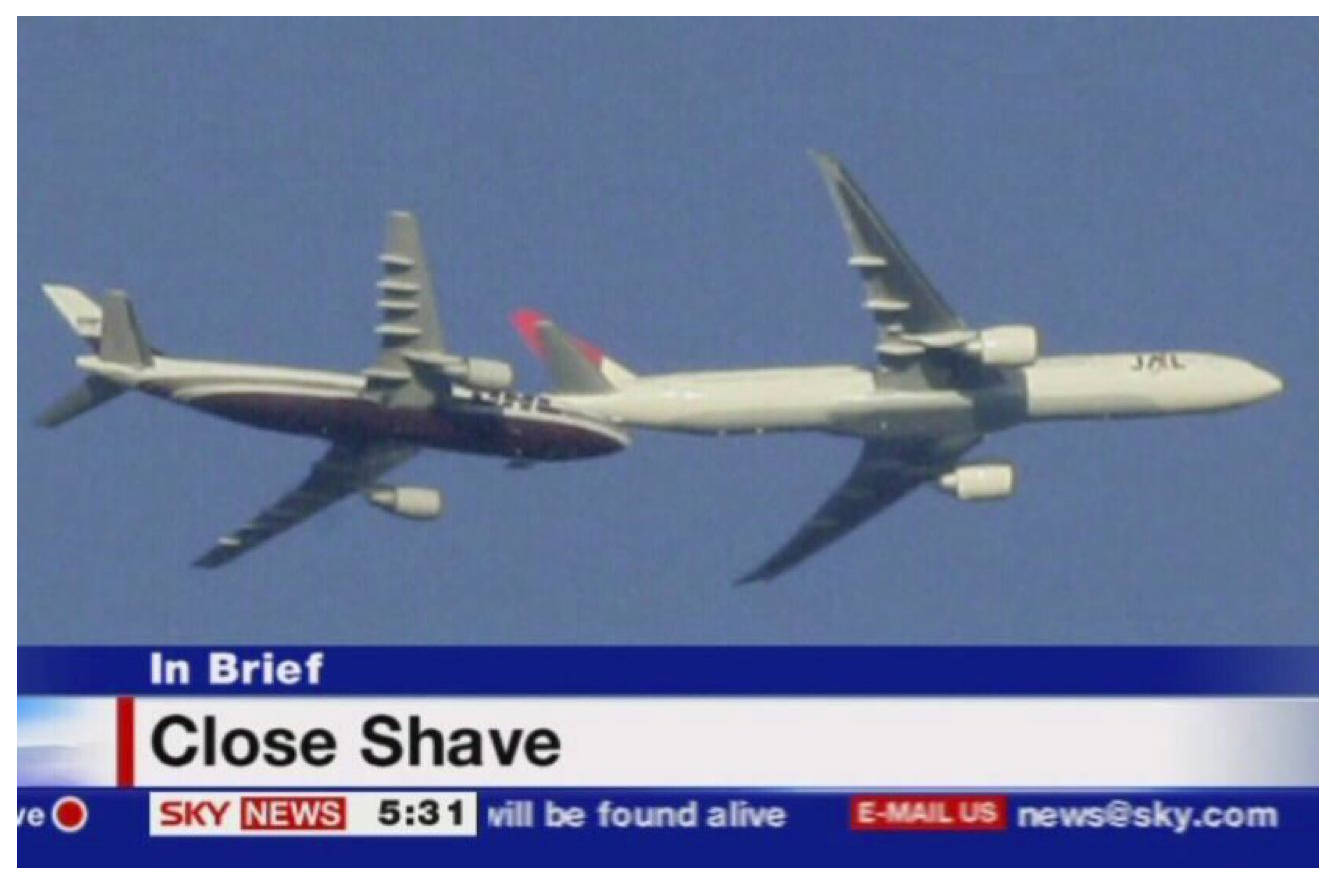
\includegraphics[angle=0,width=6.5cm]{projects/nearmiss1.eps}
\end{minipage}
%\begin{center}
%\includegraphics[angle=0,width=4cm]{2_planes.eps}
%\end{center}

\vspace{12pt}
The relative sizes of the planes in the photo can provide some information
about the {\em ratio} of the distances to the planes from the observer.
However, (i) the planes are not identical, and (ii) they are viewed at
different angles. Because of (ii) the length of the plane's
body in the photograph appears smaller than if the body is perpendicular to
the line of sight.\\[6pt]
Examine the top view of the plane (a) and its schematic kite-like
representation (b) in the diagram below. For common commercial aircraft, the
length HT and wingspan LR can be found easily. When the plane is seen at an
angle, as in diagram (c), the angle $\alpha $ between HT and LR is no
longer 90$^\circ $. The ratio of the visible wingspan, L$'$R$'$ to the visible
body length H$'$T$'$ is also different from what they are in (b).
\begin{center}
%\includegraphics[angle=-90,width=11cm]{plane_kite.pdf}
\includegraphics[angle=0,width=11cm]{projects/plane_kite.eps}
\end{center}
The task is to use the values of L$'$R$'$, H$'$T$'$ and $\alpha $
measured on the photograph, to determine what LR and HT  should be on
the photograph. One can then use this information (and the real aircaft
dimensions) to estimate how far apart the aircraft were, assuming that we
know the distance to one of them (e.g., 2 km, as the photo was taken with a
tele lens).


%\section{Walking like a pendulum}
%%\item
%\underline{\large\bf Modelling walking through a pendulum model} \\[0.1cm]
In biomechanics and robotics, walking is often modelled through
an (inverted) pendulum model. Walking is most energy efficient when
gravity dominates the movement of the legs. Under this assumption,
estimate the normal speed of walking. How would the model change
when the model of a leg is extended to include a foot or a knee?


\section{Ellipse and its normals\\ \small{(Pathway: Any; Pre-requisite: None)}}
\section{Ellipse and its normals\\ \small{(%Pathway: Any; 
Pre-requisite: None)}}
An ellipse can be defined by its equation in Cartesian coordinates
$$\frac{x^2}{a^2}+\frac{y^2}{b^2}=1,$$
where $a$ and $b$ ($b\leq a$) are its semimajor and semiminor axes,
respectively. Alternatively, it can be defined in the parametric form by
$x=a\cos t$, $y=b\sin t$, $0\leq t\leq 2\pi$.\\[6pt]
How many {\em normals} to the ellipse can you draw from a given point in the
$xy$ plane? [The normal is a line perpendicular to the tangent at the point
where it meets the curve.]


\section{Bouncing ball\\ \small{(Pathway: AMA; Pre-requisite: Classical mechanics)}}
\section{Bouncing ball\\ \small{(%Pathway: AMA; 
Pre-requisite: Classical mechanics)}}
A small ball is released from rest from a point above a large sphere
of radius $R$. If this point lies on the vertical line through the centre
of the sphere, the ball will keep bouncing along this line. However, if the
point is some distance $d$ away from this line ($d<R$), the ball will
bounce off at an angle after colliding with the sphere. In this case it will
only make a finite number of bounces on the spherical surface, before
jumping off it.\\[6pt]
Estimate the number of times the ball will bounce off the sphere.
[You may assume that the collisions are perfectly elastic. It might be
easier to find an estimate for $d\ll R$. However, an exact (numerical?)
solution may also be possible in the general case.]


 


\section{What's the angle between your vertebrae?\\ \small{(Pathway: Any; Pre-requisite: None)}}
\section{What's the angle between your vertebrae?\\ \small{(%Pathway: Any; 
Pre-requisite: None)}}
%\item
%\underline{\large\bf Measuring angles on X-ray images}  \\[0.1cm]
\begin{minipage}{9.5cm}
Using X-rays, one can measure angles between bones in a body (e.g., between
two vertebrae, as shown on the X-ray of a model with pins [1]). However, when
measuring an angle on an image, the result may not be the same as the true
angle. Thus, in the diagram below the angle $\varphi $ that an object
(``stick'' of length $l$) makes with the horizontal, is not necessarily equal
to the angle $\psi $ between its image I and the horizontal line on the
screen.
\end{minipage}
\hspace{0.3cm}
\begin{minipage}{6.5cm}
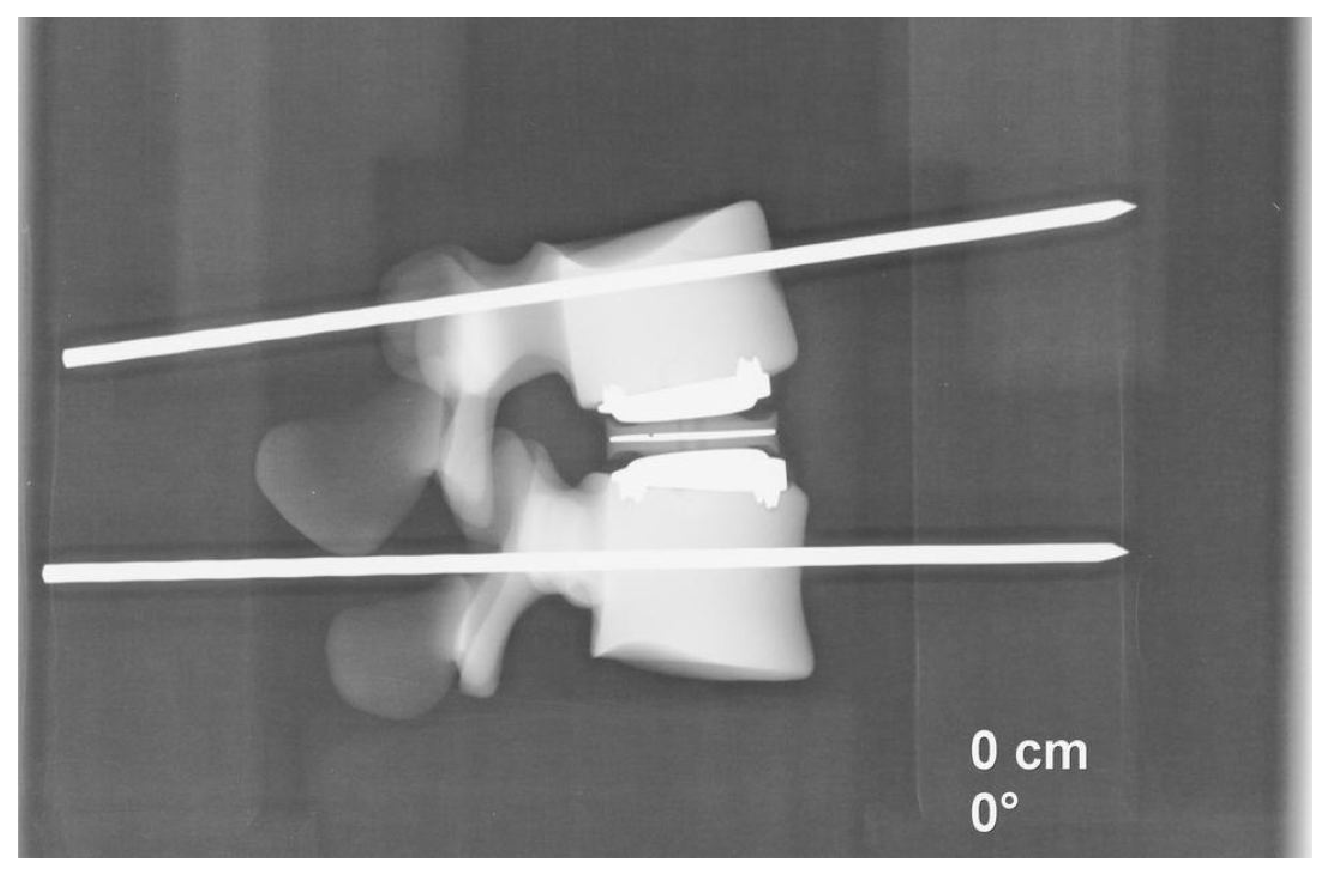
\includegraphics[angle=0,width=6.5cm]{projects/Vertebrae_image.eps}
\end{minipage}

\begin{center}
%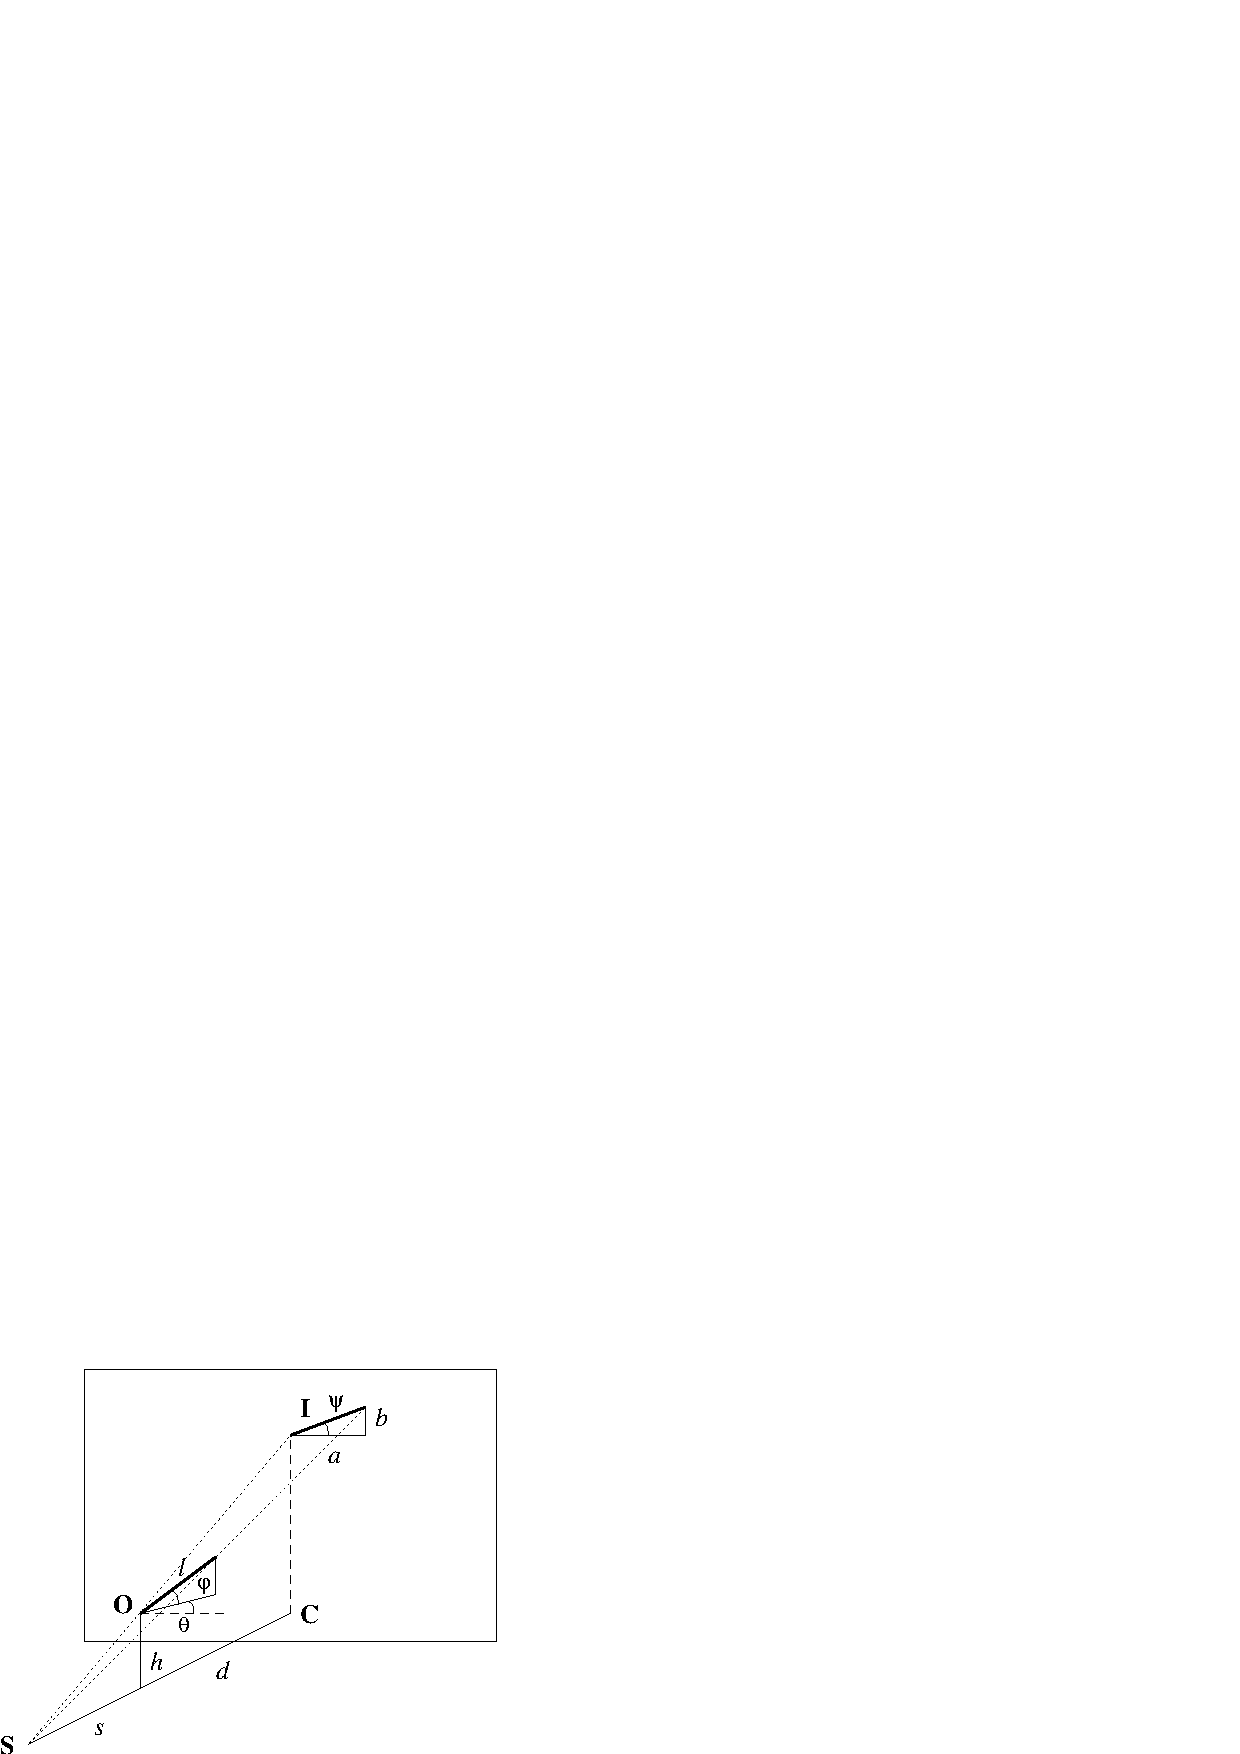
\includegraphics[width=10cm,angle=-90]{X_ray.pdf}
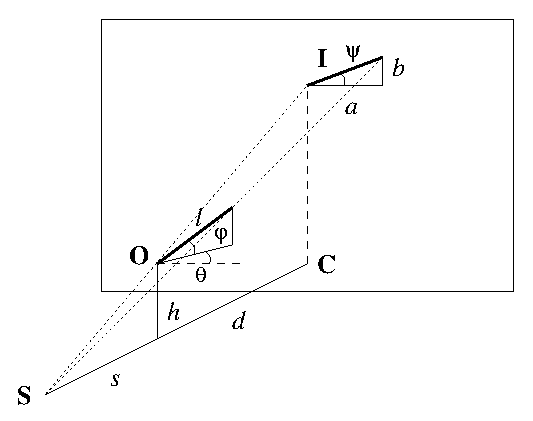
\includegraphics[width=8cm]{projects/X_ray.eps}
\end{center}

The difference between $\varphi $ and $\psi $ may depend on the
distance $s$ between the X-ray source S and the plane
parallel to the screen which contains one end of the object O,
and the distance $d$ between O and the plane of the screen.
It may also depend on the height $h$ of the end-point O
above the line SC perpendicular to the screen, and on the
angle $\theta $ that the vertical plane through O makes
with the direction parallel to the screen.\\[6pt]
Using the above diagram or otherwise, show that
\begin{equation}
\tan \psi =\frac{1}{\cos \theta }\tan \varphi -\frac{h}{s}\tan \theta .
\end{equation}
Investigate how the difference beteeen $\psi $ and $\varphi $ depends on the
angle $\theta $ and the vertical displacement $h$.\\[6pt]
You can further investigate if one can find $\varphi $ from the results of
two measurements (yielding $\psi _1$ and $\psi _2$), corresponding to two
position $\theta _1$ and $\theta _2$, for which only the difference
$\Delta \theta =\theta _2-\theta _1$ is known.\\[6pt]
[1] John McManus, {\em The Influence of X-Ray Technique on the Angle
Measurement of an Artificial Disc}, Thesis (Queen's University Belfast, 2006).
%thesis(unpublished).
%In this work X-rays were taken of model vertebrae which had metal pins
%inserted in them for the purpose of measuring the angles more accurately
%(something that would be hard to do on a real patient!).


\section{Two ships at anchor\\ \small{(Pathway: Any; Pre-requisite: None)}}
\section{Two ships at anchor\\ \small{(%Pathway: Any; 
Pre-requisite: None)}}
% Milkmaid problem
Two ships, A and B, are at anchor some distance from each other and from 
shore. A boat launched from A takes a number of crew ashore and then sails
to B. What is the quickest path the boat can take?\\[6pt]
Start by considering the simplest case of a straight shoreline. Then consider
other shapes. Can you find equations that would solve the problem in the
general case?\\[6pt]
If you want to look at a more difficult problem, add a sea current parallel
to the shore!


\section{Double pendulum\\ \small{(Pathway: AMA; Pre-requisite: Classical Mechanics)}}
\section{Double pendulum\\ \small{(%Pathway: AMA; 
Pre-requisite: Classical Mechanics)}}
% Double pentulum
A double pendulum is a pendulum with a second pendulum attached to it. We
assume that each pendulum consists of a mass $m$ at the end of a massless rod
of length $\ell$. Their positions are described by the angles $\phi _1$
and $\phi _2$ that each pendulum makes with the vertical.\\[6pt]
The Lagrangian of the system reads (verify!)
$$
L=\frac 12m\ell^2\left[2\dot\phi _1^2+\dot\phi _2^2+2\dot\phi _1\dot\phi _2
\cos(\phi _1-\phi _2)\right]+mg\ell(2\cos\phi _1+\cos\phi _2) 
$$

\begin{enumerate}\setlength{\itemsep}{0pt}
\item List the conserved quantities.
\item Describe qualitatively the motion of the pendulums with simple initial
conditions, e.g., one at rest and the other one with some initial velocity.
\item Write Lagrange's equations of motion for the variables $\phi _i$.
Investigate the motion for small $\phi _i$.
\item Use the Runge-Kutta [1] method to solve the equations of motion for
arbitrary initial conditions, using python or a programming language of your
choice.
\item Test your program with the initial conditions you discussed in 2 and
comment.
\end{enumerate}

[1] See for example: R. L. Burden and J. D. Faires, {\it Numerical Analysis}




\section{Ladybird lost\\ \small{(Pathway: Any; Pre-requisite: Classical mechanics would help, but really none)}}
\section{Ladybird lost\\ \small{(%Pathway: Any; 
Pre-requisite: Classical mechanics would help, but really none)}}
%Ladybird
In a round room of radius $R$, a large number of coins $N$ of diameter $d$ are
randomly dispersed upon the floor. A ladybird starts from the centre of the
room, crawling at speed $v$.
\begin{enumerate}\setlength{\itemsep}{0pt}
\item How long (on average) does it take before it meets a coin?
\item Suppose that every time the ladybird meets a coin, it changes direction at
random. How long (on average) before it makes it to the wall?
\item Suppose every time it `hits' a coin, the coin magically disappears.
Work out (approximately, and on average) the law of decrease of the number
of remaining coins as a function of time. (Assume that if, in the process,
the ladybird hits the wall, it is simply `reflected' back towards
the interior of the room, at a random angle.)
\item Calculate the answers for parts 1--3 for a room of typical size,
1p coins and $v = 1$~cm/s, and $N$ of your choice.
\end{enumerate}

{\it Keywords:} to work on this problem, you will need to think (or read)
about mean free paths, random walks/diffusion/Brownian motion.

%Extensions: one can ask many fun questions involving the above key words.
%Suggest one or two.


\section{Paper-scissors-stone\dots\ and jelly babies!\\ \small{(Pathway: Any, with a little bias to SOR; Pre-requisite: None, but willingness to code)}}
\section{Paper-scissors-stone\dots\ and jelly babies!\\ \small{(%Pathway: Any, with a little bias to SOR; 
 Pre-requisite: None, but willingness to code)}}
%paper-scissors-stone
Four children play a long sequence of paper-scissors-stone games in
pairs. They divide up 40 jelly babies, starting with 10 each.\\[6pt]
The eldest child begins the sequence by choosing an opponent at
random, then the next eldest chooses at random, and so on, to complete the round
of 4 games. If a child wins a game, the loser gives the winner a jelly
baby. If the game is a draw no sweets are exchanged. In each game, there is
an equal probability of winning, losing or drawing.\\[6pt]
There are two versions of the rules:
\begin{itemize}\setlength{\itemsep}{0pt}
\item[(a)] If a child, at any time, has no sweets, they are eliminated.
\item[(b)] If a child with no sweets plays a child with sweets, they
automatically win.
\end{itemize}
Carry out a computer simulation of the game.\\[6pt]
For case (a) find out how long (how many rounds), on average,
the game lasts. How does the duration of the game vary with the
number of children and the number of sweets?\\[6pt]
For case (b) find out the fraction of time the oldest child has no
sweets, and the fraction of time when they have all the sweets. Can you
explain these values mathematically?


\section{Finding the truth in TEQs\\ \small{(Pathway: SOR; Pre-requisite: None but willingness to code a bit)}}
\section{Finding the truth in TEQs\\ \small{(%Pathway: SOR; 
Pre-requisite: None but willingness to code a bit)}}
%TEQ
One of the questions that students answer when filling in Teaching Evaluation
Questionnaires (TEQ) is about the percentage of lectures they attended. After
tallying, these results (in simplified form) are presented in a table like
this
\setlength{\extrarowheight}{3pt}
\begin{center}
\begin{tabular}{|l|c|c|c|c|}
\hline
\% of lectures attended & 25\% & 50\% & 75\% & 100\% \\
\hline
No. of answers & 7 & 19 & 42 & 29 \\
\hline
\end{tabular}
\end{center}
where the total number of answers is 97.\\[6pt]
Since the TEQs are filled in in a lecture, the frequencies in the table
above are \textit{biased}. Using the data from the table, estimate the true
frequencies that would be observed if the TEQ were filled by all 150 students
in the class. You can assume that attendances by individual students are
uncorrelated random variables. Using your result, check whether the attendance
of the lecture where TEQ was taken, was typical for the given class size.\\[6pt]
Generalise your approach to an arbitrary number of scores, and to a continuous
distribution.
In each case, determine the mean and standard deviation od the number of
students in class based on the true frequencies that you obtain from the
frequencies observed in the lecture.


\section{Narrow escape\\ \small{(Pathway: Any; Pre-requisite: None)}}
\section{Narrow escape\\ \small{(%Pathway: Any; 
Pre-requisite: None)}}
%man and dog
A circular field is surrounded by a fence. A man standing in the
centre of the field can run with speed $v$. A dog can run along the fence
with speed $u=4v$. Will the man be able to escape, i.e., reach a point
in the fence before the dog gets there? (The dog and the man can
see each other at all times, and the dog is doing its best to catch the man.)
What strategy/path should the man follow?\\[6pt]
What is the maximum ratio $u/v$ for the which the man can escape? If the ratio
is greater than this, where can the man be at the start, relative to the dog, so
that he can still escape?


\section{Optimal paths through trellis networks\\ \small{(Pathway: Any; Pre-requisite: None)}}
%Optimal paths through trellis networks
Alice, Bob, Chris and Diana want to cross a bridge at night. The bridge is not
lit, but they have one torch amongst them. However, only at most two people
can cross the bridge at the same time and the torch is needed to cross the
bridge. Furthermore, Alice takes 20 minutes, and Bob 25, whereas Chris and
Diana only need 5 and 10 minutes, respectively. What is the shortest time it
takes for all four of them to cross the bridge?\\[6pt]
Can you think of a general approach to solving this problem? How would this
general approach work when Eve has to cross the bridge as well, and would
take 15 minutes to do so?\\[6pt]
One systematic way in which this problem can be solved is through trellis
graphs. Trellis networks play an important role in communication technology,
and are also used in algorithms, for example,  for finding most likely
sequences in hidden Markov models. Trellis networks can, for example, be
used for error correction techniques in digital communication through
so-called Viterbi decoding. An introduction to Viterbi decoding can be
found in many textbooks; a detailed example of such decoding is given in
[1].\\[6pt]
[1] T. K. Moon, {\it Error correction coding: mathematical methods and
algorithms} (2005).


\section{Assigning investigations\\ \small{(Pathway: Any with a little bias for SOR; Pre-requisite: None)}}
\section{Assigning investigations\\ \small{(%Pathway: Any with a little bias for SOR; 
Pre-requisite: None)}}
%Assigning Investigations

In order to be assigned an investigation project from a list, students
in a module are asked for their 5 choices without particular preferences.
You are faced with the task of assigning each student one of the projects of
their choice in a way that no two students are assigned the same topic
(\textit{satisfiability problem}). Assume that the number of projects $K$ is
greater than or equal to the number of students $N$. Devise an algorithm based
on backtracking or other forms of search that finds a feasible solution to this
problem. Discuss examples.\\[6pt]
Assume now that the 5 students' choices are ordered from their best
preference to the least one. In this case use the Hungarian algorithm, or
any other of your choice, to find the assignment that maximises the overall
students' preferences. Discuss the adequacy of 5 preferences for assigning
projects and the relationship between the number of students and number of
projects available. (Note that some projects can be much more popular
than others).


\section{Lenz's potentials\\ \small{(Pathway: AMA; Pre-requisite: Classical Mechanics)}}
\section{Lenz's potentials\\ \small{(%Pathway: AMA; 
Pre-requisite: Classical Mechanics)}}
% Lenz's potentials 
For a particle moving in a central field $U(r)$, the path can be found using
plane polar coordinates $r$ and $\phi $ in terms of an indefinite integral
[1]. However, there are only a handful of potentials for which this integral
and the equation of the path can be found analytically. You are familiar with
one example, namely the gravitational potential $U(r)=-\alpha /r$, in which
the paths are conic sections (ellipse, parabola or hyperbola). Using this
as a starting point, investigate the paths of the particle with zero energy
($E=0$) in {\it Lenz's potential}
\[
U(r)=-\frac{2uR^2}{r^2\left[\Bigl(\dfrac{r}{R}\Bigr)^\mu +
\Bigl(\dfrac{R}{r}\Bigr)^\mu \right]^2},
\]
where $u$, $R$ and $\mu $ are constants, for different values of $\mu $.
Such potentials find some unexpected applications in atoms and clusters
[V. N. Ostrovsky, Phys. Rev. A {\bf 56}, 626 (1997)].\\[6pt]
[1] L. D. Landau and E. M. Lifshitz, \textit{Mechanics}
(Butterworth-Heinemann, Oxford, 2001).



\section{Milk and Coffee\\ \small{(Pathway: Any; Pre-requisite: None)}}
There are two jugs of equal volume, one containing coffee and one milk. You take one cup of milk, pour it in the jug of coffee and mix. Then you take one cup from the mixture and pour it back into the jug of milk. 
\\
Prove that the amount of milk in the jug of coffee is the same as the amount of coffee in the jug of milk. Discuss the assumptions to arrive at this conclusion.
\\
\\
Now consider again the two jugs, one of pure milk and one of pure coffee. By transferring back and forth a cup of liquid from the first to the second jug and vice versa, is it possible to obtain two equal mixtures, i.e. two jugs containing each half coffee--half milk?
\\
\\
Discuss extensions to the problems, for instance, 3 jugs (coffee, milk and hot-chocolate), jugs of different sizes....



\section{Minds swapping\\ \small{(Pathway: Any; Pre-requisite: None)}}
\section{Minds swapping\\ \small{(%Pathway: Any; 
Pre-requisite: None)}}
A long time ago in a galaxy far, far away, four friends, Amy, Bob, Charlie and David found a strange device capable of swapping the minds of the two people using it. At first the group find it amusing, in fact Amy swapped with Bob, Charlie swapped with David and finally Amy (in Bob's body) swapped with Charlie.
\\ \\
Unfortunately, they soon realised that the device would not swap back a pair that already used the device.
Can the 4 friends swap back their minds to their original bodies?
\\ \\
Two other friends Eliza and Francis go and help their four friends. Is there a sequence of swaps that brings everybody to their original bodies avoiding a pair using the device twice?
\\ \\
Can the problem be solved when $N$ bodies are shuffled?\\
 How many swaps are needed?
\\ Discuss possible extensions.


%\pagebreak

\section{``Impossible'' exam question\\ \small{(Pathway: Any; Pre-requisite: None)}}
\section{``Impossible'' exam question\\ \small{(%Pathway: Any; 
Pre-requisite: None)}}
% Impossible economics exam
% Insert 
% \usepackage[colorlinks,urlcolor=blue]{hyperref}
% in the preamble of the main file


In January 2015, some final year economics students at Sheffield University
claimed that their exam contained an ``impossible question'' [1]. However,
the question, which is reproduced below, should give no trouble
to a mathematics student! Moreover, you should also be able to find ways of
extending it.

% Include the question exactly as it appeared on that exam, as a picture
%
%\includegraphics*[angle=0,width=15cm]{sheffieldeconomics.jpg}
%
% or use the text below.

\vspace{12pt}

{

Consider a country with many cities and assume that there are $N>0$ people in
each city. Output per person is $\sigma N^{0.5}$ and there is a coordination
cost per person of $\gamma N^2$. Assume that $\sigma >0$ and $\gamma >0$.

\begin{itemize}
\item[(a)] What sort of things does the coordination cost term $\gamma N^2$
represent? Why does it make sense that the exponent on $N$ is greater than 1?
\hfill[10 marks]

\item[(b)] Draw a graph of per-capita consumption as a function of $N$ and
derive the optimal city size $N$. How does it depend on the parameters $\sigma $
and $\gamma $? Provide intuition for your answers.\hfill[10 marks]

\item[(c)] Describe which combinations of $\sigma $ and $\gamma $ generate a
peasant economy, meaning an economy with no cities (or 1-person cities). Why
might the values of the parameters $\sigma $ and $\gamma $ have changed over
time? What do these changes imply in terms of the optimal city size?
\hfill[10 marks]

\end{itemize}
}

[1] \href{http://www.bbc.com/news/education-31057005}{http://www.bbc.com/news/education-31057005}.


\section{Design a robot\\ \small{(Pathway: Any; Pre-requisite: None)}}
\section{Design a robot\\ \small{(%Pathway: Any; 
Pre-requisite: None)}}
%\item
%\underline{\large\bf Stiff differential equations} \\[0.1cm]
\begin{minipage}{13cm}
Consider a planar mechanism which consists of three bars connected by joints (see diagram). Bars $OA$ and $O'B$ (called cranks) are free to rotate about fixed points $O$ and $O'$, respectively. Find how the coordinates of point $C$ depend on the angle $\phi$ that rod $OA$ makes with the line $O'O$. Explore how the shape of the path described by point $C$ depends on the lengths of the cranks $a$ and $b$, and lengths $c$ and $d$, taking them as fractions of the length l between points $O$ and $O'$.
In particular, if this mechanism is to model the motion of a foot, find the optimal lengths that would make point $C$ move in a curve, part of which is close to a straight line (foot in contact with the ground), the other part being an arc-like path of the foot though the air.
\end{minipage}
\hspace{0.3cm}
\begin{minipage}{4.5cm}
\includegraphics[angle=0,width=4.5cm]{projects/robota}
\end{minipage}
%\vspace{6pt}
%\begin{wrapfigure}[15]{R}{6.2cm}
%\raisebox{0pt}[\dimexpr\height-01.2\baselineskip\relax]{\includegraphics*[width=6cm]{robota}}%
%\end{wrapfigure}



\end{document}

%%%%%%%%%%%%%%



\begin{enumerate}

\item
\underline{\bf The Dirac delta function and entropy of harmonic oscillators} \hfill {\em Dr.\ Alavi} 
\\[0.1cm]
The Dirac delta function $\delta(x)$ appears in many branches of mathematical physics.  It has a number of
formal properties, including
\begin{eqnarray}
\delta(x) & = & 0 \hspace*{0.5cm} (x \neq 0) \\[0.2cm]
\int_{- \infty}^{\infty} \delta(x) ~  dx & = & 1 \\[0.2cm]
\int_{- \infty}^{\infty} \delta(x-x_0) ~ f(x)~ dx & = & f(x_0) \\[0.2cm]
\delta(f(x)) & = & \left| \frac{df(x)}{dx} \right| ^{-1} \delta(x-x_0) 
\end{eqnarray}
where in the last formula $x_0$ is chosen so that $f(x_0)$=0.  We are going to use the Dirac delta function
to evaluate the entropy of a system of harmonic oscillators. \\[0.2cm]
Consider an $N$ dimensional harmonic oscillator with the following Hamiltonian
\begin{displaymath}
H ~ = ~ \sum_{i=1}^N \frac{p_i^2}{2} ~ + ~ \sum_{i=1}^N \frac{x_i^2}{2}
\end{displaymath}
where $\{x_i\}$ are the coordinate variables and $\{p_i\}$ are the corresponding momenta.
\\[0.2cm]
If the system has total energy $E$, then the entropy $S$ of the system is given by
\begin{displaymath}
e^S ~ = ~ \int \delta(H-E)~dx_1dx_2...dx_Ndp_1dp_2...dp_N
\end{displaymath}
By investigating the properties of the Dirac delta function, obtain analytic formulae for $S$ as a 
function of $E$ and $N$. Show that
\begin{displaymath}
S ~ = ~ C(N) ~ + ~ (N-1) \log E
\end{displaymath}
where $C(N)$ is a constant dependent only on $N$.  Hence show that the entropy of the one-dimensional 
oscillator is independent of $E$. \\[0.2cm]
[Hint: Consider the special cases with $N$=1,2,3 respectively, before attempting the general case.]

\item
\underline{\large\bf Central quadric surfaces} \\[0.1cm]
The equation of a central quadric has the general form
\begin{displaymath}
\sum_{i=1}^3 \sum_{j=1}^3 a_{ij}(x_i - x_i^0)(x_j - x_j^0) = 1, \hspace*{0.5cm} a_{ji} = a_{ij}
\end{displaymath}
Classify these surfaces given that the determinant $|a_{ij}| \neq 0$.  \\[0.3cm]
Then consider the possible cases if $|a_{ij}|=0$. \\



\item
\underline{\large\bf Radiative transfer} \\[0.1cm]
The transfer of radiation through a star can be written
as the differential equation
\begin{eqnarray}
\frac{1}{\kappa_\lambda}\frac{{\rm d}I_\lambda}{{\rm d}s_\lambda}=
 -I_{\lambda}+S_\lambda
\nonumber
\end{eqnarray}
where $I_\lambda$ = radiation intensity at wavelength $\lambda$,
$\kappa_\lambda$ = absorption coefficient at $\lambda$, \linebreak[4]
${\rm d}s$ = path length,
$S_\lambda$ = source function.
Investigate the solution in the optically thin ($\tau_\lambda\ll 1$)
and optically thick ($\tau_\lambda\gg 1$)
limiting cases, with zero and non-zero starting values of $I_\lambda$.
\\[0.3cm]
\underline{Suggested reading}
\\
You may want to consult a text book on astrophysics for
more detailed background to this equation, eg. 
B\"{o}hm-Vitense, `Introduction to stellar astrophysics' vol. 2 (CUP, 1989). \\



\item
\underline{\large\bf Having a whale of a time}  \\[0.1cm]
The blue whale, the largest animal known to have lived on land or sea, was caught in large numbers
earlier this century and this resulted in a drastic decline in the size of the population.  
The blue whale is now officially a protected species.  However, it has been supposed that it will
become extinct in the near future because the number currently alive is so small that the males have a 
near impossible task of finding a mate. \\[0.2cm]
If the male and female populations, $M$ and $F$ respectively, are assumed, in the absence of encounters,
to decline at a rate proportional to the size of each population and the number of encounters is taken
to be proportional to $MF$, the equations determining $M$ and $F$ take the form
\begin{displaymath}
\frac{dM}{dt}~ = ~ - \alpha M ~ + ~ \beta MF
\end{displaymath}
\begin{displaymath}
\frac{dF}{dt}~ = ~ - \eta F ~ + ~ \gamma MF
\end{displaymath}
where $\alpha$, $\beta$, $\gamma$ and $\eta$ are positive constants. \\[0.2cm]
Analyse in detail the predictions this model makes about the behaviour of $M$ and $F$ with time.
Assign appropriate values to $\alpha$, $\beta$, $\gamma$ and $\eta$ and the values of $M$ abd $F$ at time
$t=0$, and use the equations to determine $M$ and $F$ at a sample range of subsequent times.  
Compare these results with any information you can obtain about the actual behaviour of the populations.
\\[0.2cm]
How would you modify the model to take into account
\begin{enumerate}
\item the effect of illegal whaling;
\item the limitation imposed on the population by the finite resources available to maintain the whales?
\end{enumerate}

\end{enumerate}

\end{document}
